\documentclass[10pt]{article}

%\documentstyle[12pt]{mystyle}

\usepackage{epsfig}
\usepackage{times}
\usepackage{amsmath}
\usepackage{amssymb}
\usepackage{fancyvrb}
\usepackage{fancyhdr}
\usepackage{graphicx}
\usepackage{color}
\usepackage[colorlinks=true,urlcolor=blue]{hyperref}
\usepackage[svgname]{xcolor}

\topmargin -0.3in
\oddsidemargin 0in
\evensidemargin 0in
\headheight 12pt
\headsep 12pt
\textheight 8.85in
\textwidth 6.5in
\parindent 0pt

\raggedbottom

\def\beqa#1\eeqa{\begin{eqnarray}#1\end{eqnarray}}
\newcommand{\R}{{\cal{R}}}
\newcommand{\N}{{\cal{N}}}
\newcommand{\C}{{\cal{C}}}
\newcommand{\D}{{\cal{D}}}
\renewcommand{\S}{{\cal{S}}}
\newcommand{\bx}{{\bf{x}}}
\newcommand{\bX}{{\bf{X}}}
\newcommand{\bt}{{\bf{t}}}
\newcommand{\bw}{{\bf{w}}}
\newcommand{\bm}{{\bf{m}}}
\newcommand{\bv}{{\bf{v}}}
\newcommand{\bS}{{\bf{S}}}
\newcommand{\bM}{{\bf{M}}}
\newcommand{\bphi}{{\boldsymbol{\phi}}}
\newcommand{\bPhi}{{\boldsymbol{\Phi}}}
\renewcommand{\d}{{\textrm{d}}}
\newcommand{\Figref}[1]{Fig.~\ref{#1}}
\newcommand{\Eqref}[1]{Eq.~\ref{#1}} % The '~' stops breaking and gives correct spacing
\newcommand{\Eqrefs}[2]{Eqs.~\ref{#1},~\ref{#2}}

\newcommand{\bh}{{\bf{h}}}
\newcommand{\ba}{{\bf{a}}}
\newcommand{\bb}{{\bf{b}}}
\newcommand{\Z}{{\cal{Z}}}
\newcommand{\bmu}{{\boldsymbol{\mu}}}
\newcommand{\bSigma}{{\boldsymbol{\Sigma}}}




\pagestyle{fancyplain}
\lhead{\fancyplain{}{Homework 3}}
\rhead{\fancyplain{}{10-707: Deep Learning}}
\cfoot{\thepage}

\title{\textsc{Homework 3}} % Title

\newcommand{\outDate}{Sept 11, 2017}
\newcommand{\dueDate}{Sept 25, 2017 11:59 pm}

\author{CMU 10-707: \textsc{Deep Learning (Fall 2017)} \\
\url{https://piazza.com/cmu/fall2017/10707} \\
OUT: Nov 1 \\
DUE: Nov 15 \\ 
TAs: Dimitris Konomis, Dheeraj Rajagopal, Yao-Hung (Hubert) Tsai} 

\date{}
\begin{document}
\maketitle
\setcounter{page}{1}

%\markboth{\hfil STA 4273H, Assignment 1}{
%          \hfil STA 4273H, Assignment 1}

%\vspace*{-32pt}

%\vspace*{9pt}

\section{Problem 1 (20 pts)}

Assume a network that computes a 4-gram language model\footnote{https://en.wikipedia.org/wiki/N-gram}, which computes $P(w_i | w_{i-1} w_{i-2} w_{i-3})$ as shown in figure \ref{fig:lm}. 
Consider a dataset of natural language sentences with a vocabulary size $V$. The network contains $H$ hidden units in the hidden layer and each word $w$ in the input $X$ is of the embedding dimension $D$. Specifically, your embedding layer will have $D*$number\_of\_words (which is three for this specific question) for this language model. In addition to the architecture in the figure, assume that the hidden layer is followed by a tanh non-linearity layer.

Assuming a softmax layer at the end with a cross-entropy loss for prediction, derive the backpropagation equations for the loss, with respect to the weights and biases shown in the figure (word embedding weights, embedding to hidden weights, hidden to output weights and their corresponding biases). While deriving, clearly mention the dimensions of each weight matrix and the bias terms. 


\section{Problem 2 (20 pts)}

\begin{figure}[h]
  \centering
  \vspace{-0.2in}
  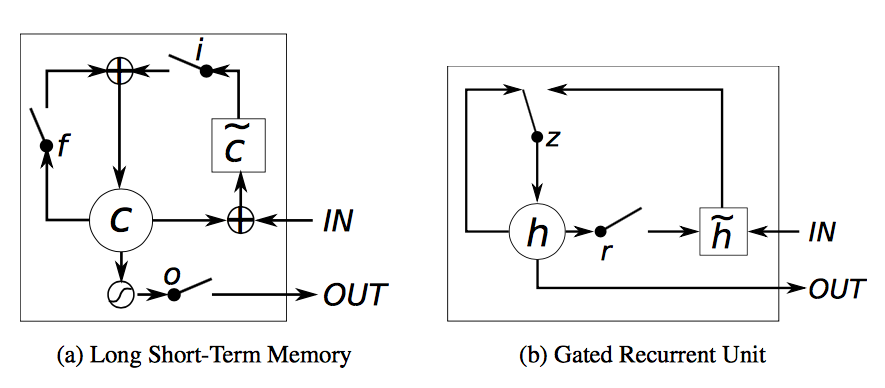
\includegraphics[width=0.8\linewidth]{lstm_gru.png}
  \vspace{-0.2in}
  \caption{Illustration of (a) LSTM and (b) GRU.}
  \label{fig:lstm_gru}
\end{figure}


Gated Recurrent Unit (GRU) is a gating mechanism similar to Long Short-term Memory (LSTM) with similar performance. 

LSTM has the following equations:
\begin{equation*}
\begin{split}
\mathbf{f}_t &= \sigma\,\big(W_f \mathbf{x}_t + U_f \mathbf{h}_{t-1} + b_f\big) \\
\mathbf{i}_t &= \sigma\,\big(W_i \mathbf{x}_t + U_i \mathbf{h}_{t-1} + b_i\big) \\
\mathbf{o}_t &= \sigma\,\big(W_o \mathbf{x}_t + U_o \mathbf{h}_{t-1} + b_o\big) \\
\tilde{\mathbf{c}}_t &= \mathrm{tanh} \,\big(W_c \mathbf{x}_t + U_c \mathbf{h}_{t-1} + b_c\big) \\
\mathbf{c}_t &= \mathbf{f}_t \odot \mathbf{c}_{t-1} + \mathbf{i}_t \odot \tilde{\mathbf{c}}_t \\
\mathbf{h}_t &= \mathbf{o}_t \odot \mathrm{tanh}\big( \mathbf{c}_t\big) ,
\end{split}
\end{equation*}
where $\odot$ is element-wise product. Note that these equations are different from the ones in the course slides. In the slides, the {\em peephole} LSTM is introduced, whereas we use a simpler version of the LSTM. For details see \cite{hochreiter1997long}.

On the other hand, GRU has the following equations:
\begin{equation*}
\begin{split}
\mathbf{z}_t &= \sigma\,\big(W_z \mathbf{x}_t + U_z \mathbf{h}_{t-1} + b_z\big) \\
\mathbf{r}_t &= \sigma\,\big(W_r \mathbf{x}_t + U_r \mathbf{h}_{t-1} + b_r\big) \\
\tilde{\mathbf{h}}_t &= \mathrm{tanh} \,\big(W \mathbf{x}_t + U (\mathbf{r}_t \odot \mathbf{h}_{t-1}) + b\big) \\
\mathbf{h}_t &= \mathbf{z}_t \odot \tilde{\mathbf{h}}_t + (\mathbf{1} - \mathbf{z}_t)\odot \mathbf{h}_{t-1}.
\end{split}
\end{equation*}

Fig. \ref{fig:lstm_gru} illustrations the architecture for LSTM and GRU. Please briefly answer the following questions:

\begin{itemize}
\item[(a)] How many gates are there in LSTM and GRU, respectively? Please also specify the names of gates in LSTM/GRU.
\item[(b)] Summarize in your own words, the functions of the gates in the GRU and LSTM, and then compare between them. 
\item[(c)] In terms of outputs (``OUT'' in Fig. \ref{fig:lstm_gru} (a) and (b)), what are the differences between LSTM and GRU? 
\item[(d)] Suppose $\mathbf{x}\in \mathbb{R}^m$ and $\mathbf{h} \in \mathbb{R}^n$ ($\mathbf{c} \in \mathbb{R}^n$), please compute the numbers of parameters in each LSTM and GRU unit, respectively.
\item[(e)] Suppose you have two networks consisting of a sequence of LSTM or GRU cells (with the same number of cells). Which networks might take less time to train and generalize? Please also explain why in a few sentences. 
\end{itemize}



\section{Problem 3 (60 pts)}

 In this problem, you are going to build a 4-gram language model using a Multilayer Perceptron with an embedding layer as in figure \ref{fig:lm}. For each of the 4 word combinations, you will predict the next word given the first three words. Please do not use any toolboxes. We recommend you use Matlab or Python, but you are welcome to use any programming language of your choice
\\
The goal is to build a 4-gram language model using a Multilayer Perceptron with an embedding layer. For each of the 4 word combinations, you will predict the next word given the first three words. 

\subsection{Data Preprocessing (10 pts)}
In this question, you will learn to preprocess the data. The dataset is given in the files \emph{train.txt} and \emph{val.txt}. Each of the files contain one sentence per line. You are required to do the following


\begin{enumerate}
\item Create a vocabulary dictionary (i.e.) you are required to create an entry for every word in the training set (make the data lower-cased). This will serve as a lookup table for the words and their corresponding id. Note: Splitting it on space should do, there is no need for any additional processing. 
\item For each sentence, include a START tag (before the sentence) and END tag (after the sentence). 
\item How many trainable parameters are in the network including the weights and biases ?
\end{enumerate}

For language models, you will often encounter the problem of finding new words in the test/validation set. You should add an additional token `UNK' in the vocabulary to accommodate this. This is also useful when you truncate your vocabulary size to avoid long-tail distributions. Everytime a word from the truncated vocabulary appears, use `UNK' instead.'

For this homework problem, limit your vocabulary size to 8000 (including the `UNK', `START' and `END'). Plot the distribution of 4-grams and their counts. Report the most common 4-grams (top 50) and your observations from the distribution graph.

\subsection{Backpropagation with Linear Hidden Layer (20 pts)}
\begin{figure}
  \centering
  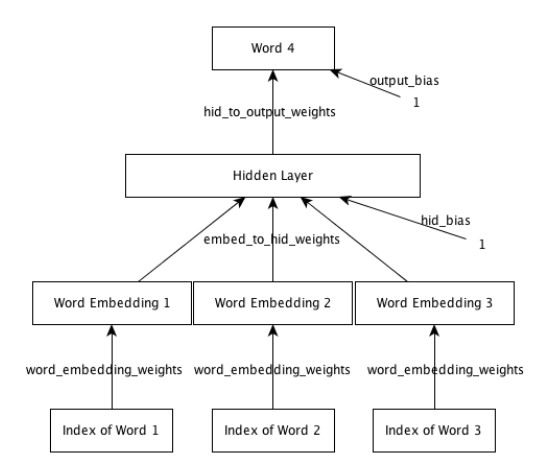
\includegraphics[width=0.6\linewidth]{lm.png}
  \caption{Language Model Architecture}
  \label{fig:lm}
%   \vspace{-0.2in}
\end{figure}

You will now implement the model shown in figure \ref{fig:lm} with the linear 
hidden layer. 
Each word will be represented by a 16-dimensional embedding followed by hidden layer of 128 units. Your network's output will be the softmax over the vocabulary which tries to predict the next word. You are going to minimize cross entropy loss between the predicted softmax and next word.
\\

For each epoch, plot your perplexity on the validation set (val.txt). Run your model for 100 epochs. Report your observation with graph of perplexity \footnote{http://www.cs.columbia.edu/~mcollins/lm-spring2013.pdf} and total loss.
\\

Also, report the same observations on the same network with 256 and 512 hidden layer units.
Note: When computing perplexity of the validation set, you will often encounter words that you have not seen in the training set.

\subsection{Incorporating Non-linearity (10 pts)}

Now, you will be adding non-linear activations after the hidden layer. Include tanh activations for the hidden layer output. Do you see any changes in the trend of loss and perplexity (compared to network without non-linearity)? Describe your findings in a few sentences and show appropriate plots (after running at least 100 epochs).

\subsection{Analysis (10 pts)}

Language Generation: Pick three words from the vocabulary that go well together (for example,‘government of united’, ‘city of new’, ‘life in the’, ‘he is the’ etc.). Use the model to predict the next ten words (or stop at the END token). What do you notice as you generate more words ? Report your findings for five such `three word' combinations. 
\\

Implement a function that computes the distance between two embeddings. Your function should compute the euclidean distance between the word vectors. Does your language model learn that the distances between similar words are smaller ? Report your findings.

\subsection{Embedding Layer Visualization (10 pts)}

Reduce the embedding dimension to 2. Retrain the whole network. Visualize the learnt embeddings for 500 randomly picked words from the vocabulary and plot in a 2-D graph. What do you observe? Do similar words appear nearby in the plot? Report your findings with the plot.


\subsection{Extra Points (10 pts)}

For extra points, you will implement the same language model but this time with a Recurrent Neural Network. This takes care of the order in which the words are given as input to the model.

Note: For this extra points question, you are allowed to use a deep learning package of your choice (PyTorch, TensorFlow, Theano, etc.)

\subsubsection{Recurrent Neural Network}
Each of the input will now go to an RNN cell that processes one word at a time and computes probabilities of the possible values for the 4-gram(time step = 4).

The input to this network should be batched with a batch size of 16.

The architecture starting from the embedding layer, hidden layer (with tanh activation) and softmax remains the same as the architecture in \ref{fig:lm} with hidden layer size = 128 and embedding size = 16.

\subsubsection{Embedding layer}
Try the following sizes for embedding dimension [32, 64, 128]. Report your findings based on cross-entropy error and perplexity of validation set.

\subsubsection{Truncated Backpropagation}
It is a usual practice to truncate backpropagation  in RNNs \cite{Williams90anefficient} for long sequences. Now, you will try truncating the backprop(to 2 words) for randomly selected 10\% of words. Plot the error and perplexity and report your findings.



\section*{Write up}
Hand in answers to all questions above. For Problem 3, 
the goal of your
write-up is to document the experiments you have done and your main findings, so
be sure to explain the results. Be concise and to the point -- do not write 
long paragraphs or only vaguely explain results. 

\begin{itemize}
\item 
The answers to all questions
should be in pdf form (please use \LaTeX).
\item Please include a README file with instructions on how to execute your code.

\item Package your code and README document using
\texttt{zip} or \texttt{tar.gz} in a file called \\
\texttt{10707-A3-*yourandrewid*.[zip|tar.gz]}. 

\item Submit your PDF write-up to the Gradescope assignment ``Homework 3" and your packaged code to the Gradescope assignment ``Code for Homework 3." 

\end{itemize}

\bibliographystyle{plain}
\bibliography{references}

\end{document}
